\chapter{Rotas do back-end}

A seguir são listadas e explicadas todas as rotas do backend.

\section{Rota raiz}

Página inicial, apresenta a lista de aeródromos para que o usuário escolha um. 
Internamente, por meio do ORM, é feita a seleção dos campos \texttt{AerodromeName},
\texttt{ICAO} e \texttt{City} e o resultado é posto em uma lista de tuplas que é 
enviada para o template.

Exemplo do resultado enviado à ferramenta de template:
\begin{smaller}
\setstretch{0.8} 
\begin{verbatim}
{
  "airports": [
  [
    "Presidente Juscelino Kubitschek",
    "SBBR",
    "Bras\u00edlia"
  ],
  [
    "Tancredo Neves",
    "SBCF",
    "Belo Horizonte"
  ],
  [
    "Afonso Pena",
    "SBCT",
    "Curitiba"
  ],
  ...
]
}
\end{verbatim}
\end{smaller}


\section{Rota: /info/\{ICAO\}}

Retorna informações de um aeródromo com o ICAO especificado na URL. São exibidos,
além da explicação do METAR atual:

\begin{itemize}
    \item Pista
        \begin {itemize}
        \item Cabeceiras
        \item Comprimento
        \item Largura.
        \end {itemize}
    \item Frequências do aeródromo (nem todos os items a seguir poderão estar disponíveis). Visualmente cada item contém o tipo a que se refere e a frequência em si.
    \begin{itemize}
        \item Torre
        \item Solo
        \item Operações
        \item Rampa
        \item Tráfego
        \item ATIS
    \end{itemize}
    \item Frequências de navegação (nem todos os items a seguir poderão estar disponíveis)
    \begin{itemize}
        \item ILS
            \begin{itemize}
                \item Qual cabeceira este ILS se refere
                \item Frequência
                \item Direção final de aproximação (CRS)
                \item Identificador (um código de três letras que este ILS é identificado nas cartas aeronauticas)
            \end{itemize}
        \item VOR
            \begin{itemize}
                \item Frequência
                \item Identificador (um código de três letras que este VOR é identificado nas cartas aeronauticas)
            \end{itemize}
    \end{itemize}
\end{itemize}

\section{Rota: /history/\{ICAO\}}
Para um aeródromo retorna informações dos dez últimos METARs em três
gráficos com o eixo horizonal sendo o tempo.

\begin{itemize}
    \item Gráfico 1
    \begin{itemize}
        \item Temperature (graus Célsius)
        \item Ponto de orvalho (graus Célsius)
    \end{itemize}
    \item Gráfico 2
    \begin{itemize}
        \item Velocidade do vento (milhas náuticas por hora)
        \item Direção do vento (graus)
    \end{itemize}
    \item Gráfico 3
    \begin{itemize}
        \item Ajuste altímetro (hectopascal)
        \item Visibilidade (metro)
    \end{itemize}
\end{itemize}

\section{Rota: /taf/\{ICAO\}}
Retorna o próximo TAF válido para este aeródromo com a explicação de cada item.

Exemplo do resultado enviado à ferramenta de template para o aeroporto do Galeão.

\begin{smaller}
\setstretch{0.8}     
\begin{verbatim}
{
   "icao":"SBGL",
   "taf":"251600Z 2518/2624 23012KT 8000 BKN020 BKN030 TN16/2609Z TX20/2615Z \n  
   TEMPO 2518/2521 23012G25KT 5000 DZ BR BKN015 BKN020 \n  TEMPO 2521/2524 25010KT 
   4000 RA BR BKN010 BKN020 \n  TEMPO 2600/2612 22008KT 3100 RA BR BKN007 BKN015 \n  
   BECMG 2612/2614 26007KT 7000 BKN016 BKN023 \n  BECMG 2618/2620 32005KT BKN017 
   RMK PGA",
   "decoded":[
      ["251600Z",
      "Disponibilizado em 16:00Z no dia 25"],
      ["2518/2624",
      "Válido do dia 25 as 18:00Z até dia 26 as 24:00Z"],
      ["23012KT",
      "Vento proa <b>230</b>° com velocidade <b>12</b> nós (kt)."],
      ["8000",
      "Visibilidade 8000 metros"],
      ["BKN020",
      "Nuvens broken (5/8 a 7/8 do céu com nuvens) em <b>2000</b> pés de altitude. "],
      ["BKN030",
      "Nuvens broken (5/8 a 7/8 do céu com nuvens) em <b>3000</b> pés de altitude. "],
      ["TN16/2609Z",
      "A temperatura mínima é de 16°C prevista de ocorrer dia 26 as 09:00 (UTC)"],
      ["TX20/2615Z",
      "A temperatura máxima é de 20°C prevista de ocorrer dia 26 as 15:00 (UTC)"],
      [
         ["TEMPO 2518/2521",
         "Condições temporárias previstas do dia 25 as 18:00 (UTC) até dia 25 as 
         21:00 (UTC)"],
         ["23012G25KT",
         "Vento proa 230° com velocidade 12 nós (kt) e <b>rajadas</b> de 25 nós."],
         ["5000",
         "Visibilidade 5000 metros"],
         ["DZ",
         "Chuvisco moderada."],
         ["BR",
         "Névoa úmida moderada."],
         ["BKN015",
         "Nuvens broken (5/8 a 7/8 do céu com nuvens) em <b>1500</b> pés de altitude. "],
         ["BKN020",
         "Nuvens broken (5/8 a 7/8 do céu com nuvens) em <b>2000</b> pés de altitude. "]
      ],
      [
         ["TEMPO 2521/2524",
         "Condições temporárias previstas do dia 25 as 21:00 (UTC) até dia 25 as 24:00 
         (UTC)"],
         ["25010KT",
         "Vento proa <b>250</b>° com velocidade <b>10</b> nós (kt)."],
         ["4000",
         "Visibilidade 4000 metros"],
         ["RA",
         "Chuva moderada."],
         ["BR",
         "Névoa úmida moderada."],
         ["BKN010",
         "Nuvens broken (5/8 a 7/8 do céu com nuvens) em <b>1000</b> pés de altitude. "],
         ["BKN020",
         "Nuvens broken (5/8 a 7/8 do céu com nuvens) em <b>2000</b> pés de altitude. "]
      ],
      ...
   ]
}
\end{verbatim}
\end{smaller}

Perceba que os grupos TEMPO e BECMG são
agrupados para que no front-end o usuário possa exibir ou ocultar cada grupo. Conforme mostram
as imagens abaixo.

\begin{figure}[ht]
    \begin{center}
    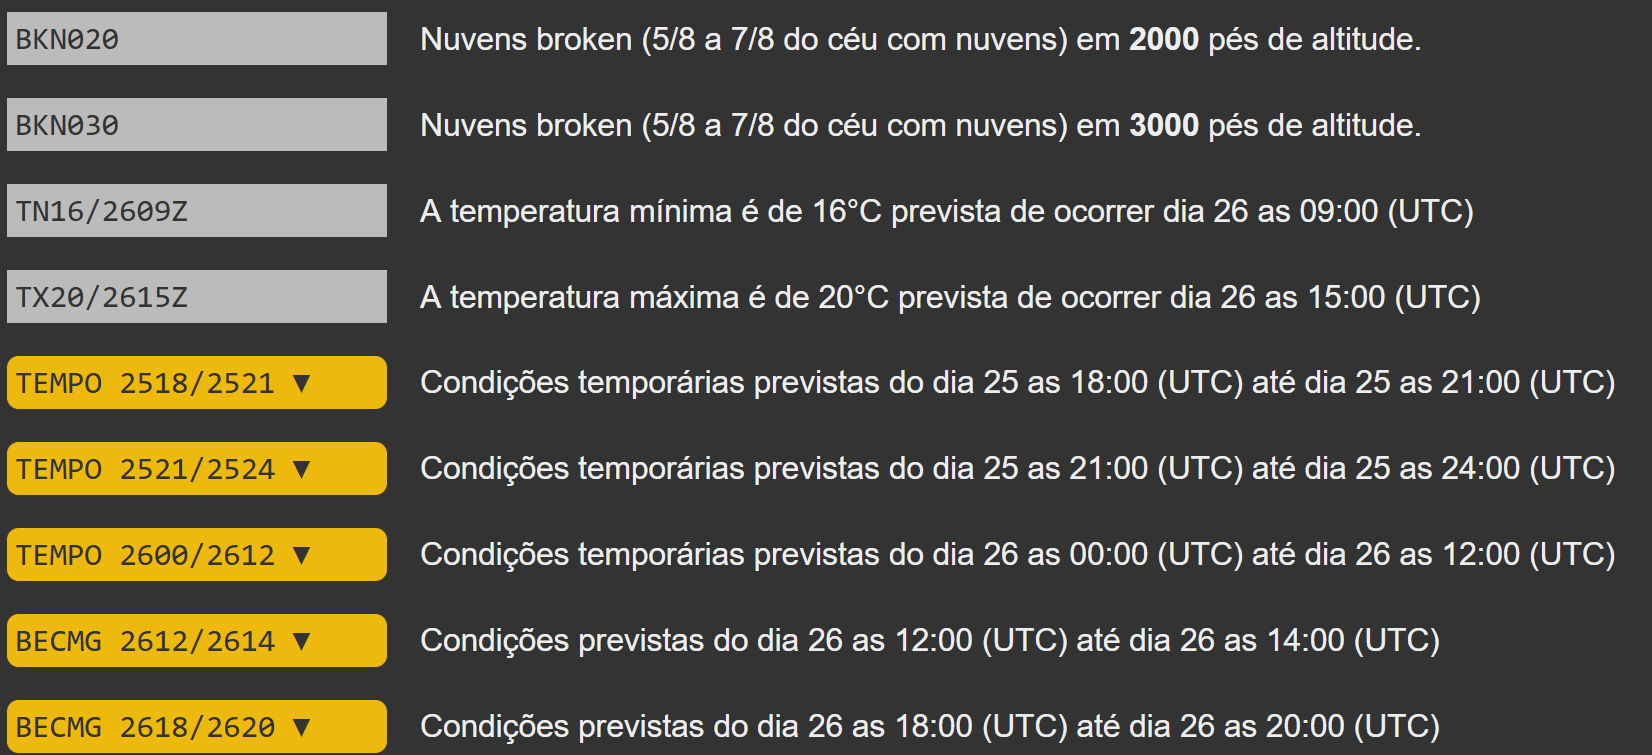
\includegraphics[width=400pt]{img/BECMG-oculto.png}
    \caption{Grupo BECMG oculto}
    \label{fig:becmg-oculto}
    \end{center}
\end{figure}

\begin{figure}[ht]
    \begin{center}
    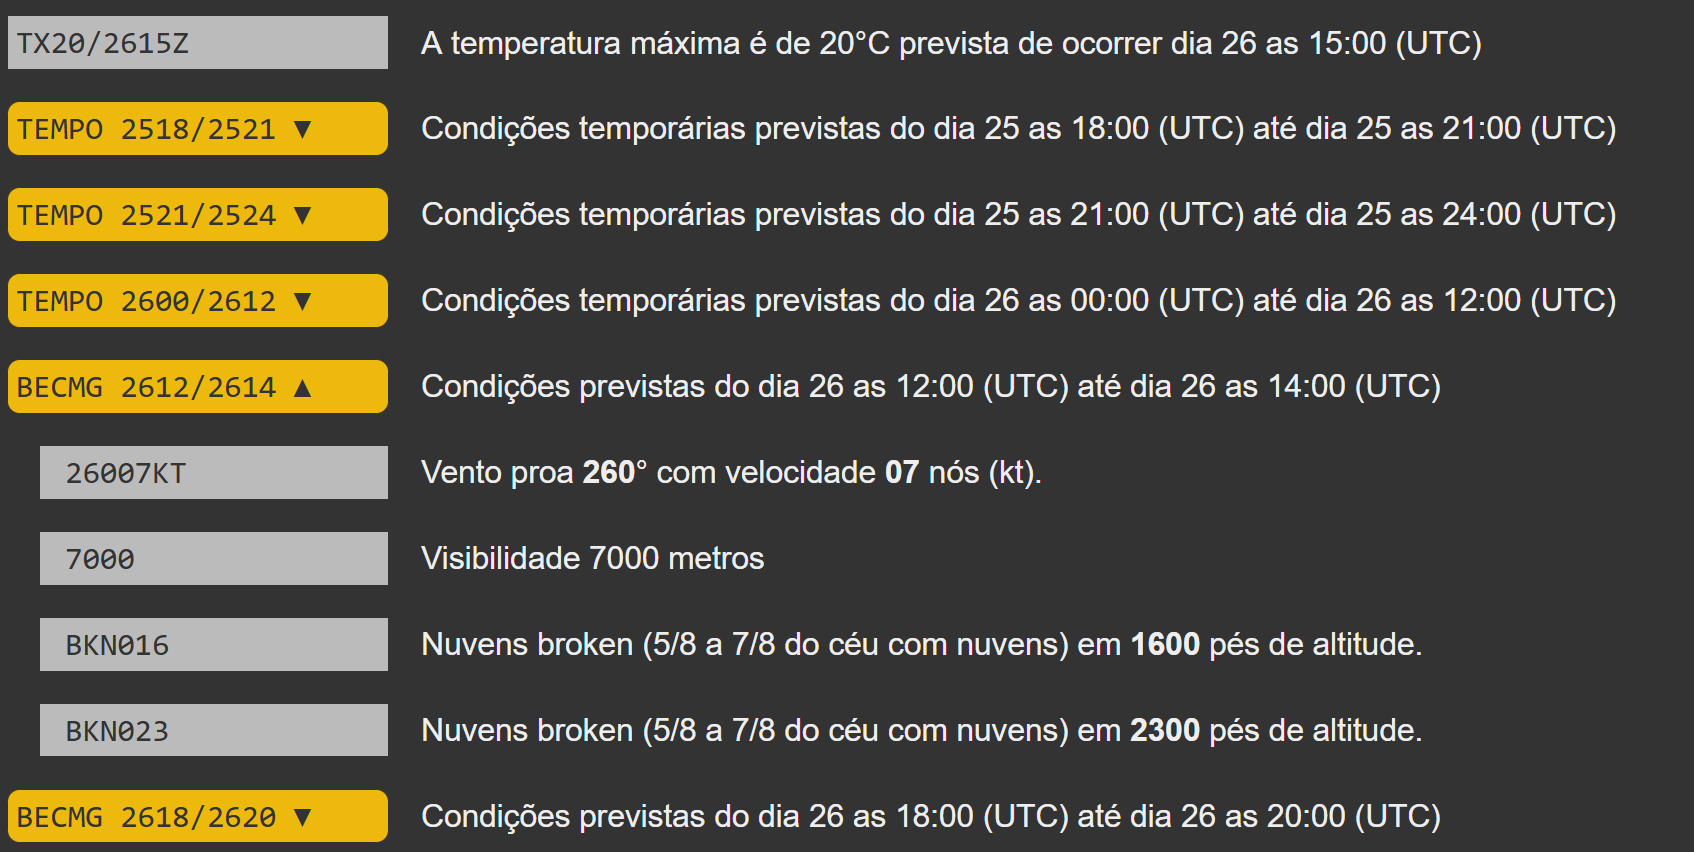
\includegraphics[width=400pt]{img/BECMG-exibido.png}
    \caption{Grupo BECMG exibido}
    \label{fig:becmg-exibido}
    \end{center}
\end{figure}


